\documentclass[tikz,border=10pt]{standalone}
\usepackage{amsmath}
\usepackage{pgfplots}
\usepgfplotslibrary{groupplots}
\pgfplotsset{compat=1.18}
\definecolor{ink}{HTML}{21352F}
\definecolor{teal}{HTML}{087F7B}
\definecolor{blue}{HTML}{4B77A8}
\definecolor{gold}{HTML}{C58B2A}

\begin{document}
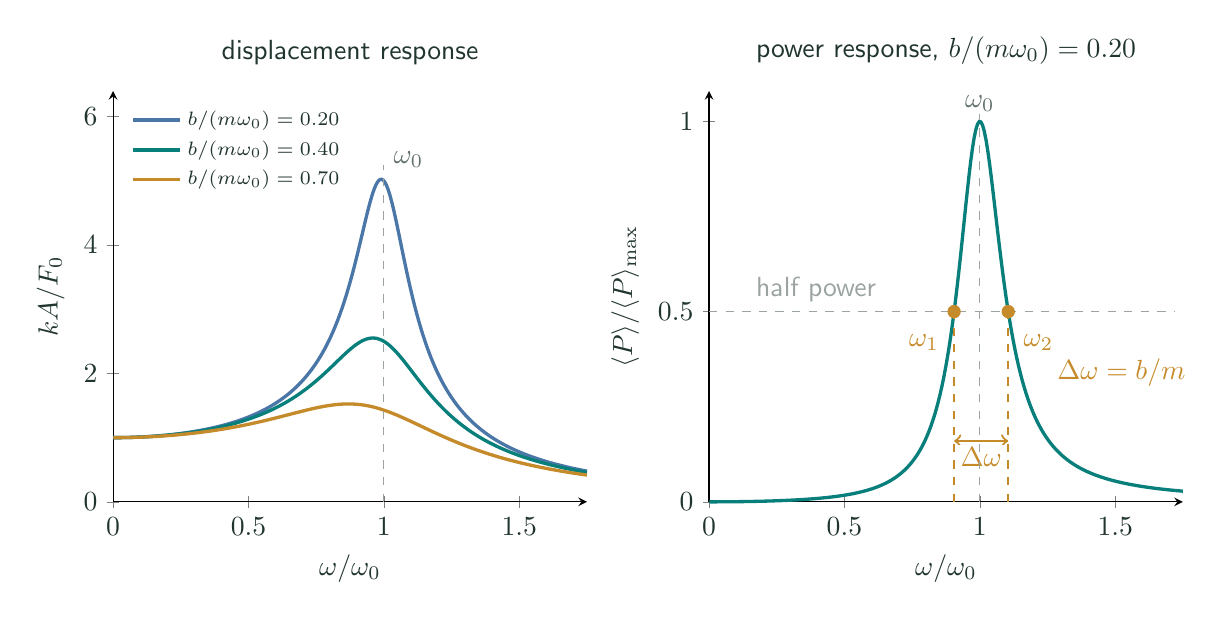
\begin{tikzpicture}[font=\sffamily,text=ink]
  \pgfmathsetmacro{\damping}{0.20}
  \pgfmathsetmacro{\halfLow}{sqrt(1+(\damping/2)^2)-\damping/2}
  \pgfmathsetmacro{\halfHigh}{sqrt(1+(\damping/2)^2)+\damping/2}

  \begin{groupplot}[
    group style={group size=2 by 1,horizontal sep=1.55cm},
    width=7.6cm,height=6.8cm,
    axis lines=left,
    xmin=0,xmax=1.75,
    xlabel={$\omega/\omega_0$},
    samples=280,
    domain=.001:1.75,
    clip=false
  ]
    \nextgroupplot[
      ymin=0,ymax=6.4,
      ylabel={$kA/F_0$},
      title={displacement response},
      legend style={draw=none,font=\scriptsize,at={(.02,.98)},anchor=north west}
    ]
      \addplot[blue,very thick]
        {1/sqrt((1-x^2)^2+(0.20*x)^2)};
      \addlegendentry{$b/(m\omega_0)=0.20$}
      \addplot[teal,very thick]
        {1/sqrt((1-x^2)^2+(0.40*x)^2)};
      \addlegendentry{$b/(m\omega_0)=0.40$}
      \addplot[gold,very thick]
        {1/sqrt((1-x^2)^2+(0.70*x)^2)};
      \addlegendentry{$b/(m\omega_0)=0.70$}
      \draw[ink!45,dashed] (axis cs:1,0)--(axis cs:1,5.25);
      \node[ink!70,above right] at (axis cs:1,5.05) {$\omega_0$};

    \nextgroupplot[
      ymin=0,ymax=1.08,
      ylabel={$\langle P\rangle/\langle P\rangle_{\max}$},
      title={power response, $b/(m\omega_0)=0.20$},
      ytick={0,.5,1}
    ]
      \addplot[teal,very thick]
        {(\damping^2*x^2)/((1-x^2)^2+\damping^2*x^2)};
      \draw[ink!45,dashed]
        (axis cs:0,.5)--(axis cs:1.72,.5)
        node[pos=.23,above] {half power};
      \draw[gold,thick,dashed]
        (axis cs:\halfLow,0)--(axis cs:\halfLow,.5);
      \draw[gold,thick,dashed]
        (axis cs:\halfHigh,0)--(axis cs:\halfHigh,.5);
      \addplot[only marks,mark=*,mark size=2.2pt,gold]
        coordinates {({\halfLow},.5) ({\halfHigh},.5)};
      \node[gold,below left=2pt] at (axis cs:\halfLow,.48) {$\omega_1$};
      \node[gold,below right=2pt] at (axis cs:\halfHigh,.48) {$\omega_2$};
      \draw[<->,gold,thick]
        (axis cs:\halfLow,.16)--(axis cs:\halfHigh,.16)
        node[midway,below=1pt,fill=white,inner sep=1pt] {$\Delta\omega$};
      \node[gold,anchor=west] at (axis cs:1.25,.34)
        {$\Delta\omega=b/m$};
      \draw[ink!45,dashed] (axis cs:1,0)--(axis cs:1,1.02);
      \node[ink!70,above] at (axis cs:1,1.0) {$\omega_0$};
  \end{groupplot}
\end{tikzpicture}
\end{document}
